% section3_1_posterior.tex — Module B: Bo
% Addresses QHM Core Task 1, §3.3 (MCMC sampling) and §3.4 (interpretation).
\subsection{Posterior Inference}\label{sec:posterior}

Combining the likelihood~\eqref{eq:likelihood} with the priors~\eqref{eq:priors} yields the joint posterior $p(\boldsymbol{\beta},\sigma\mid\mathbf{y},\mathbf{X})$ over $(\beta_0,\beta_1,\beta_2,\sigma)$. This posterior admits no closed form: the joint presence of three coefficients and an unknown residual scale precludes the Normal--Normal conjugacy available in the single-coefficient known-variance case. We therefore approximate it by Markov chain Monte Carlo (MCMC).

\paragraph{MCMC configuration (Core Task~1, §3.3)}

Sampling was performed with the No-U-Turn Sampler (NUTS), a self-tuning variant of Hamiltonian Monte Carlo, as implemented in \texttt{PyMC}~5. We ran $C=4$ independent chains with $W=1{,}000$ warm-up iterations and $T=2{,}000$ retained iterations per chain, producing $S=CT=8{,}000$ posterior samples. The warm-up phase serves a dual role: NUTS adapts its step size and diagonal mass matrix during this phase, and the corresponding draws are simultaneously discarded as burn-in, so no further explicit burn-in is removed. The target acceptance probability was set to $\alpha=0.95$ (above the default $0.80$) to suppress divergent transitions; none were reported. The random seed was fixed at $42$, matching the data-subsampling seed of Module~A, so that the entire pipeline is reproducible from raw data to posterior summaries.

\paragraph{Convergence diagnostics}

Two standard diagnostics confirm that the four chains have converged to a common posterior distribution. First, the potential scale reduction factor satisfies $\hat{R}=1.00$ for every parameter, well below the conventional warning threshold of $1.01$. Second, the bulk effective sample size satisfies $N_{\text{eff}}^{\text{bulk}}\in[3{,}775,\,5{,}371]$ across the four parameters, exceeding the rule-of-thumb minimum of $400$ recommended for stable estimation of central tendency. A more detailed treatment of trace plots and autocorrelation is deferred to Section~\ref{sec:sampler}; the present subsection therefore proceeds directly to posterior inference.

\paragraph{Posterior summaries}

Table~\ref{tab:posterior} reports, for each parameter $\theta\in\{\beta_0,\beta_1,\beta_2,\sigma\}$, the posterior mean $\hat{\theta}=\operatorname{\mathbb{E}}[\theta\mid\mathbf{y}]$, the posterior standard deviation, and the 95\% highest-density credible interval (HDI). The HDI is preferred over an equal-tailed interval because it always contains the most plausible parameter values and remains meaningful for asymmetric posteriors. Marginal posterior densities of all four parameters are shown in Figure~\ref{fig:post_density}; each is approximately symmetric and unimodal.

\begin{table}[htbp]
\centering\small
\caption{Posterior summaries based on $S=8{,}000$ NUTS samples ($4$ chains $\times\ 2{,}000$ retained draws). All $\hat{R}=1.00$ and bulk ESS exceeds $3{,}500$ for every parameter.}
\label{tab:posterior}
\begin{tabular}{lrrrrrr}
\hline
Parameter & Mean & SD & 95\% HDI low & 95\% HDI up & ESS bulk & $\hat{R}$ \\
\hline
$\beta_0$ (intercept)        & $2541$  & $382$           & $1799$  & $3324$  & $3{,}775$ & $1.00$ \\
$\beta_1$ ($x_{i1}$, temp.)  & $6784$  & $436$           & $5915$  & $7632$  & $5{,}371$ & $1.00$ \\
$\beta_2$ ($x_{i2}$, hum.)   & $-2350$ & $555$           & $-3457$ & $-1276$ & $4{,}181$ & $1.00$ \\
$\sigma$                     & $1500$  & $\phantom{0}56$ & $1393$  & $1610$  & $5{,}352$ & $1.00$ \\
\hline
\end{tabular}
\end{table}

\begin{figure}[htbp]
\centering
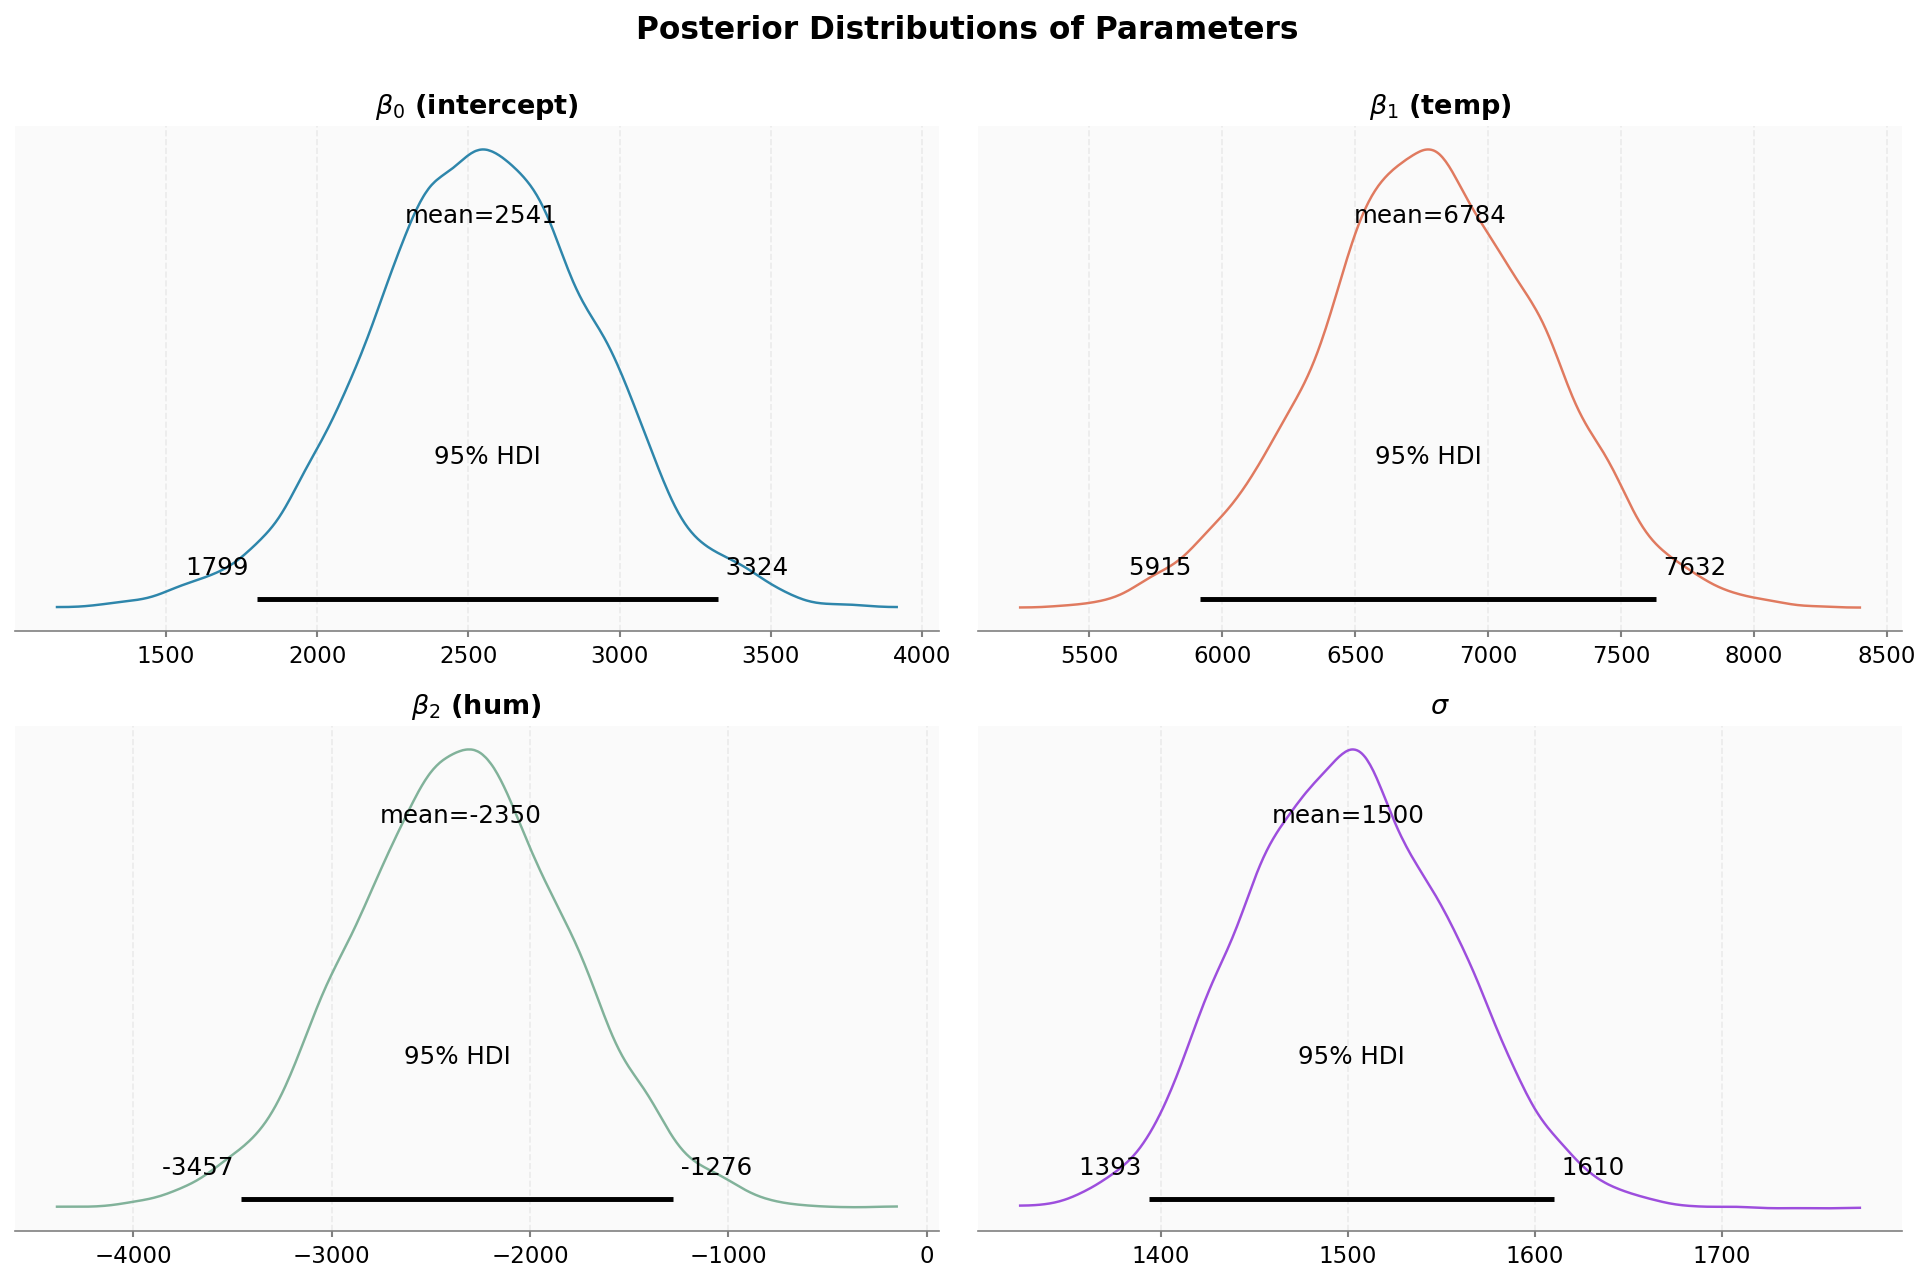
\includegraphics[width=0.6\textwidth]{../results/figures/posterior_density.png}
\caption{Marginal posterior densities of $\beta_0,\beta_1,\beta_2,\sigma$; the bar beneath each curve marks the 95\% HDI.}
\label{fig:post_density}
\end{figure}

\paragraph{Substantive interpretation (Core Task~1, §3.4)}

Coefficient interpretations refer to the normalised covariate scale: a unit change in $x_{i1}$ corresponds to the full empirical temperature swing ($-8$ to $39^{\circ}\text{C}$, a $47^{\circ}\text{C}$ range), and a unit change in $x_{i2}$ corresponds to the full humidity swing (from arid to saturated air).

\textbf{Temperature ($\beta_1$).} The posterior mean is $\hat{\beta}_1=6784$ with 95\% HDI $(5915,\,7632)$. The lower limit exceeds zero by more than $13$ posterior standard deviations, so the posterior probability $\Pr(\beta_1>0\mid\mathbf{y})$ is effectively unity. A unit increase in normalised temperature is associated, on average, with approximately $6{,}800$ additional daily rentals, identifying temperature as the dominant explanatory mechanism in the model.

\textbf{Humidity ($\beta_2$).} The posterior mean is $\hat{\beta}_2=-2350$ with 95\% HDI $(-3457,\,-1276)$. The exclusion of zero from this interval supports the conclusion that humidity meaningfully suppresses bike-sharing activity, in agreement with the negative slope visible in the exploratory analysis of Section~\ref{sec:introduction}. The wider interval relative to that of $\beta_1$ reflects both the weaker correlation in the data and the smaller absolute effect.

\textbf{Intercept ($\beta_0$).} The posterior mean is $\hat{\beta}_0=2541$ with 95\% HDI $(1799,\,3324)$. Under the parametrisation in~\eqref{eq:likelihood}, $\beta_0$ represents the expected daily count when both predictors are simultaneously zero — a corner of the predictor space not realised in the data, retained for completeness rather than substantive interpretation.

\textbf{Residual scale ($\sigma$).} The posterior mean is $\hat{\sigma}=1500$ with 95\% HDI $(1393,\,1610)$. The relative scale $\hat{\sigma}/\bar{y}\approx 0.34$ indicates that temperature and humidity together leave roughly one third of the daily standard deviation of $y$ unexplained, consistent with the modest coefficient of determination $R^{2}=0.405$ obtained from the OLS baseline. This residual variation is attributable to calendar effects, holidays, and other meteorological covariates that are deliberately omitted in order to retain the two-predictor specification dictated by the project scope.
